\begin{figure*}[t]
\centering
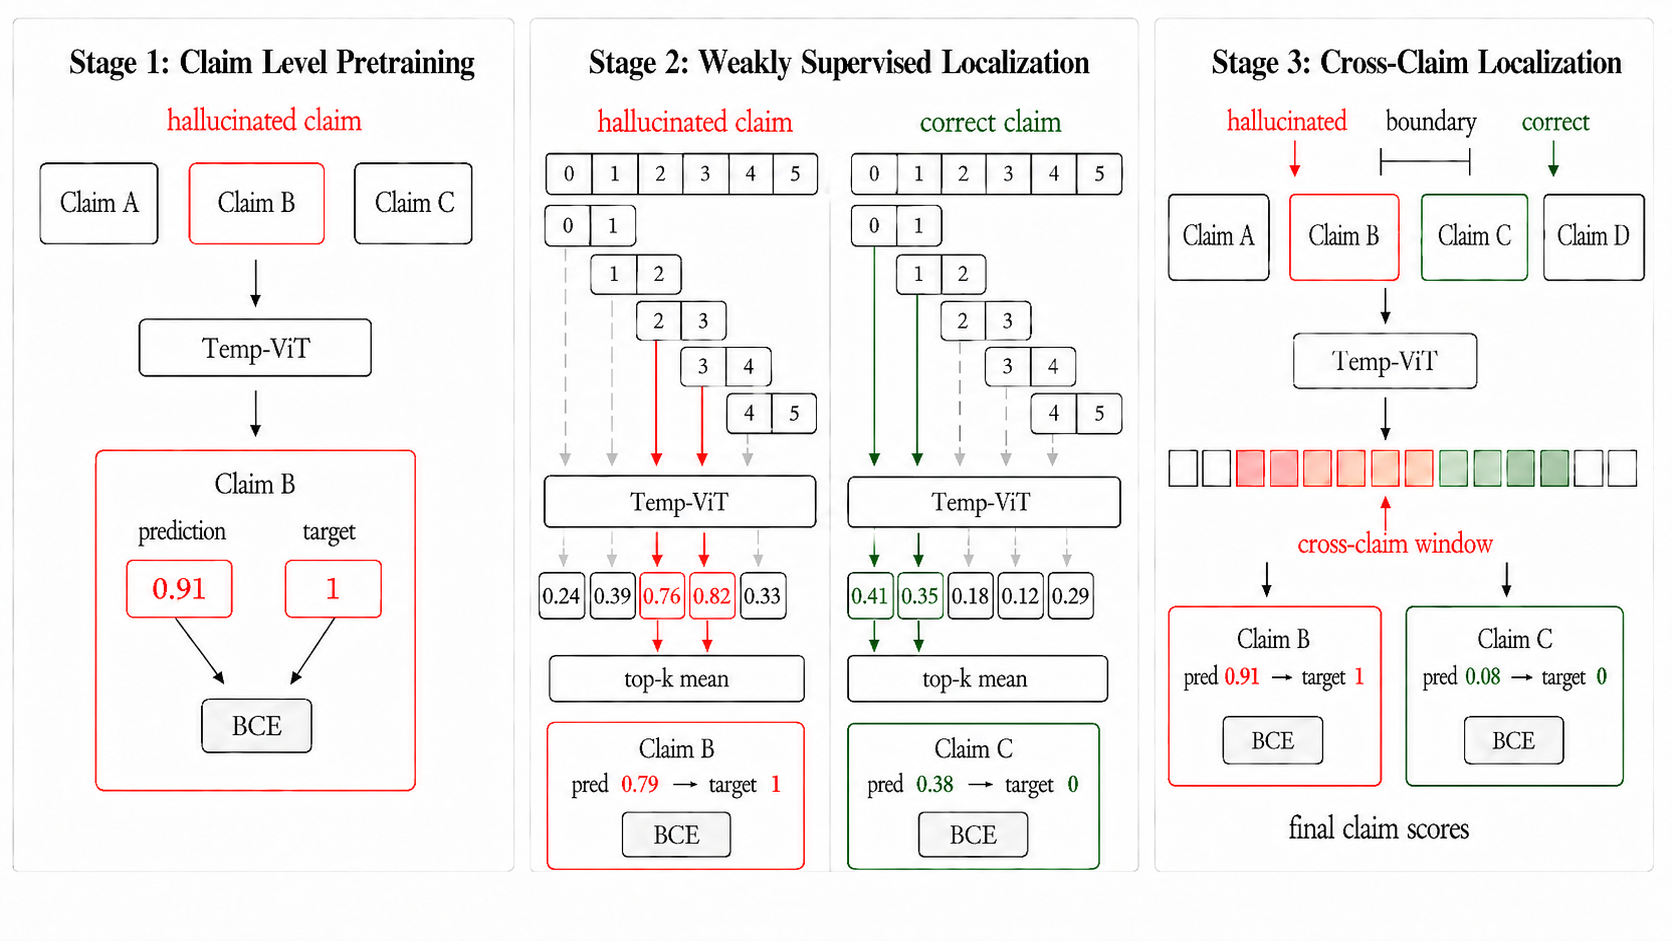
\includegraphics[width=0.95\linewidth]{figs/fig1_overview.png}
\caption{Three-stage Temp-ViT.
\textbf{Stage~1} (top): an ACT-ViT encoder maps a per-atom activation
tensor $A \in \mathbb{R}^{L \times T \times D}$ to an atom-level
uncertainty score via Pool $\to$ per-LLM linear adapter $\to$ ViT
$\to$ linear head.
\textbf{Stage~2} (middle): the encoder is frozen and applied to
centered length-$W$ token windows; a Mamba-2 temporal head emits one
logit per window, aggregated by top-$k$ MIL into an atom-level score.
\textbf{Stage~3} (bottom): the head is fine-tuned on whole passages
with noisy per-atom labels $\tilde{y}_m$ from atomic-fact
verification; per-token logits are smoothed and aggregated within
each atom span $(\ell_m, r_m)$ via a per-atom BCE, so the head ranks
uncertainty across atoms rather than scoring each in isolation.}
\label{fig:overview}
\end{figure*}
